\chapter{Samples}
\index{Library!Components!samples}
\index{Samples|textbf}
\label{c:samples}

This class of components models the sample of the experiment.
This is by far the most challenging part of an xray scattering
instrument to model. However, for purpose of simulating
instrument performance, details of the samples are rather unimportant,
allowing for simple approximations. On the contrary, for full
virtual experiments it is of importance to have realistic and
detailed sample descriptions. \MCX\ contains both simple and detailed
samples.

An important component class is elastic Bragg scattering from an ideal powder.
The component \textbf{PowderN} models a powder scatterer with reflections
given in an input file. 
The component includes absorption, incoherent scattering, direct beam
transmission and can assume \emph{concentric} shape, i.e. can be used
for modelling sample enviroments.

Next type is Bragg scattering from single crystals. Two types of single crystal exist in \MCX
at present: The \textbf{Perfect\_crystal} and \textbf{Single\_crystal} components.
\textbf{Perfect\_crystal} is in fact most often used as a monchromator crystal. It models a 
crystal where peak broadening is dominated by the Darwin width. Currently it only handles a
single defined reflection. If more than one is wanted this could be
accomplished by using two instances in a \texttt{GROUP} and dynamically choose between
them with a \texttt{WHEN}-statement. For details on the \texttt{GROUP} and \texttt{WHEN} constructs see the
main \MCX user manual~\cite{mcxtracemanual}

Much more general, the component \textbf{Single\_crystal}
is a single crystal sample (with multiple scattering) that allows
the input of an arbitrary unit cell and a list of structure factors, read
from a LAZY / Crystallographica file.
This component also allows anisotropic mosaicity
and $\Delta d/d$ lattice space variation.

Isotropic small-angle scattering is simulated in \textbf{Saxs\_Spheres},
which models scattering from a collection of hard spheres (dilute colloids).
Furthermore, a whole series of sample components modelling various SAXS standard 
sample types are available in the  \texttt{contrib} component library section.

\subsection{Scattering notation}
In sample components, we use a notation common for scattering experiments,
where the wave vector transfer is denoted the {\em scattering vector}
\begin{equation} \label{eq:q-transfer}
\boldsymbol{q} \equiv \boldsymbol{k}_\mathrm{i} - \boldsymbol{k}_\mathrm{f} .
\end{equation}
In analygo, the {\em energy transfer} is given by
\begin{equation} \label{eq:w-transfer}
\hbar \omega \equiv E_\mathrm{i} - E_\mathrm{f} =
\frac{\hbar^2}{2 m_\mathrm{n}} \left( k_\mathrm{i}^2 - k_\mathrm{f}^2 \right) .
\end{equation}

\subsection{Weight transformation in samples; focusing}

Within many samples,
the incident beam is attenuated by scattering and absorption,
so that the illumination varies considerably throughout the sample.
For single crystals, this phenomenon is known as
{\em secondary extinction} \cite{bacon}, but the effect is
important for all samples.
In analytical treatments, attenuation is difficult to deal with,
and is thus often ignored, making a {\em thin sample approximation}.
In Monte Carlo simulations, the beam attenuation
is easily taken care of, as will be shown below.
In the description, we ignore multiple scattering, which is however
 implemented in some sample components.

The sample has an absorption cross section per unit cell of
$\sigma_c^a$ and a scattering cross section per unit cell
of $\sigma_c^s$. The x-ray path length
in the sample before the scattering event is denoted by $l_1$, and
the path length within the sample after the scattering
is denoted by $l_2$, see figure \ref{powderFig}.
We then define the inverse penetration lengths as
$\mu^s = \sigma_c^s / V_c$ and $\mu^a = \sigma_c^a / V_c$, where
$V_c$ is the volume of a unit cell. Physically, the attenuation
along this path follows
\begin{equation}
f_\mathrm{att}(l) = \exp(- l (\mu^s + \mu^a)) ,
\end{equation}
where the normalization $f_\mathrm{att}(0)=1$.

\begin{figure}
  \begin{center}
    \psfrag{l1}{$l_1$}
    \psfrag{l2}{$l_2$}
    \psfrag{lfull}{$l_\mathrm{full}$}
    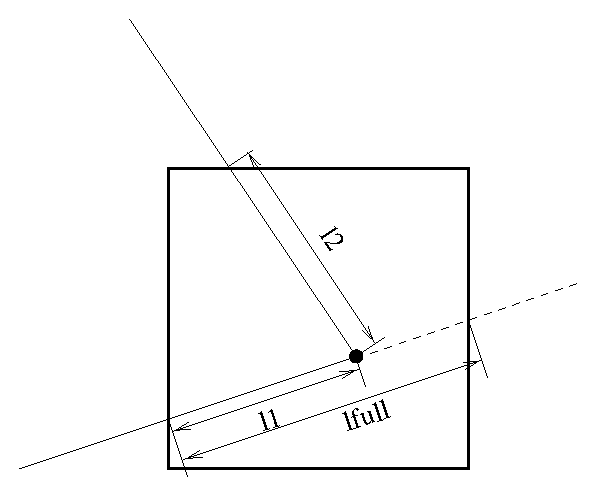
\includegraphics[width=0.6\textwidth]{figures/scatter.eps}
  \end{center}
\caption{The geometry of a scattering event within a powder sample.}
\label{powderFig}
\end{figure}

The probability for a given x-ray to be scattered from within the interval
$[ l_1 ; l_1+dl ]$ will be
\begin{equation}
P(l_1) dl = \mu^s f_\mathrm{att}(l_1) dl ,
\end{equation}
while the probability for a x-ray to be scattered from within
this interval into the solid angle $\Omega$ {\em and}
not being scattered further
or absorbed on the way out of the sample is
\begin{equation}
P(l_1,\Omega) dl d\Omega =
  \mu^s f_\mathrm{att}(l_1) f_\mathrm{att}(l_2) \gamma(\Omega) d\Omega dl ,
\end{equation}
where $\gamma(\Omega)$ is the directional distribution
of the scattered x-rays, and $l_2$ is determined by
Monte Carlo chocies of $l_1$, $\Omega$,
and from the sample geometry, see e.g. figure \ref{powderFig}.

In our Monte-Carlo simulations, we may choose the scattering
parameters by making a Monte-Carlo choice of $l_1$ and $\Omega$
from a distribution different from $P(l_1,\Omega)$.
By doing this, we must adjust $\pi_i$ according to
the probability transformation rule (\ref{probrule}).
If we {\em e.g.}\ choose the scattering depth, $l_1$,
from a flat distribution in $[ 0 ; l_\mathrm{full} ]$,
and choose the directional dependence from $g(\Omega)$,
we have a Monte Carlo probability
\begin{equation}
f(l_1,\Omega) = g(\Omega) / l_\mathrm{full} ,
\end{equation}
$l_\mathrm{full}$ is here the path length through the sample
as taken by a non-scattered x-ray (although we here
assume that all simulated x-rays are being scattered).
According to (\ref{probrule}), the x-ray weight factor
is now adjusted by the amount
\begin{equation}     \label{sampleprob}
\pi_i(l_1,\Omega) =
 \mu^s l_\mathrm{full} \exp \left[ - (l_1+l_2) (\mu^a + \mu^s) \right]
  \frac{\gamma(\Omega)}{g(\Omega)} .
\end{equation}

In analogy with the source components, it is possible to define
"interesting" directions for the scattering.
One will then try to focus the scattered x-rays,
choosing a $g(\Omega)$, which peaks around these directions.
To do this, one uses (\ref{sampleprob}), where the
fraction $\gamma(\Omega)/g(\Omega)$ corrects for the focusing.
One must choose a proper distribution so that
$g(\Omega) > 0$ in every interesting direction. If this is not the
case, the Monte Carlo simulation gives incorrect results.
All samples have been constructed with a focusing
and a non-focusing option.


\subsection{Future development of sample components}
There is still room for much more development of functionality in
\MCX\ samples.

%\input{vanadium.tex}         \newpage
%\input{tunneling.tex}        \newpage
\section{Absorption\_sample: An absorption phantom}
\index{Samples!Absorption}
\index{Tomography}
\label{absorption_sample}
\mcdoccomp{samples/Absorption_sample.parms}

This component models an absorption phantom with a single inclusion in surrounding material. It is intended use
is for tomographic imaging simulations.

%describe data format
 
\newpage
\section{Saxs\_spheres: A model of dilute hard spheres in solution for SAXS-use}
\index{Samples!SAXS}
\index{Samples!Dilute colloid medium}
\index{Diffraction}
\index{Small angle scattering}
\label{saxs_spheres}

\mcdoccomp{samples/Saxs_spheres.parms}

%The component {\bfseries Sans\_spheres} models a sample of small independent
%spheres of radius $R$, which are uniformly distributed
%in a rectangular volume $x_w \times y_h \times z_t$ with a volume
%fraction $\phi$. The absorption cross section density for the spheres
%is $\sigma_a$ (in units of m$^{-1}$), specified
%for neutrons at 2200 m/s. Absorption and incoherent scattering
%from the medium is neglected.
%The difference in scattering length density
%(the contrast) between the hard spheres and the medium is called $\Delta \rho$.
%$d$ denotes the distance to the (presumed circular) SANS detector of radius $R$.
%
%A usage example of this component can be found in the \verb+Neutron site/tests/SANS+ instrument from the \verb+mcgui+.
%
%\subsection{Small-angle scattering cross section}
%The neutron intensity scattered into a solid angle $\Delta \Omega$
%for a flat isotropic SANS sample in transmission geometry
%is given by \cite{ILLblue}:
%\begin{equation}
%I_s(q) = \Psi \Delta\Omega T A z_\mathrm{max} \frac{d\sigma_v}{d\Omega}(q) ,
%\end{equation}
%where $\Psi$ is the neutron flux, $T$ is the sample transmission,
%$A$ is the illuminated sample area, and $z_\mathrm{max}$ the length of
%the neutron path through the sample.
%
%In this component, we consider only scattering from a thin solution
%of monodisperse hard spheres of radius $R$, where the volume-specific
%scattering cross section is given by \cite{ILLblue}
%\begin{equation}
%\frac{d\sigma_v}{d\Omega}(q) =
%  n (\Delta\rho)^2 V^2 f(q)  ,
%\end{equation}
%where $f(q) = \left( 3\frac{\sin(qR)-qR\cos(qR)}{(qR)^3} \right)^2$,
%$n$ is the number density of spheres, and $V = 4 / 3 \pi R^3$ is the
%sphere volume. (The density is thus $n = \phi/V$.)
%
%Multiple scattering is ignored.
%
%\subsection{Algorithm}
%All neutrons, which hit the sample volume, are scattered.
%(Hence, no direct beam is simulated.)
%For scattered neutrons, the following steps are taken:
%\begin{enumerate}
%\item Choose a value of $q$ uniformly in the interval $[0;q_\mathrm{max}]$.
%\item Choose a polar angle, $\alpha$,
%  for the {\bfseries q}-vector uniformly in $[0;\pi]$.
%\item Scatter the neutron according to $(q,\alpha)$.
%\item Calculate and apply the correct weight factor correction.
%\end{enumerate}
%
%\subsection{Calculating the weight factor}
%The scattering position is found by a Monte Carlo choice uniformly
%along the whole (unscattered) beam path with the sample, length $l_\mathrm{full}$, giving
%$f_l = 1/l_\mathrm{full}$. The direction focusing on the detector gives
%(in an small angle approximation) $f_\Omega = d^2 / (\pi R_\mathrm{det}^2)$.
%
%Hence, the total weight tranformation factor becomes % (more explanation to come)
%\begin{equation}
%\pi_j = l_\mathrm{full} (\pi R_\mathrm{det}^2 / d^2)/(4 \pi)
%  n (\Delta\rho)^2 V^2 f(q) \exp(-\mu_a l) ,
%\end{equation}
%where $\mu_a$ is the linear attenuation factor due to absorption
%and $l$ is the total neutron path length within the sample.
%
%This component does NOT simulate absolute intensities. This latter depends on the detector parameters. \index{Bugs}
%
%Some alternative implementations exist as contributed components.
%
%The \verb+SANS+ test/example instrument exists in the distribution for this component.
 \newpage
\section{PowderN: A general powder sample}
\index{Samples!Powder, multiple diffraction line}
\index{Diffraction}
\index{Sample environments}
\index{Concentric components}
\label{powder}

\section{PowderN: A general powder sample}
\index{Samples!Powder, multiple diffraction line}
\index{Diffraction}
\index{Sample environments}
\index{Concentric components}
\label{powder}

\section{PowderN: A general powder sample}
\index{Samples!Powder, multiple diffraction line}
\index{Diffraction}
\index{Sample environments}
\index{Concentric components}
\label{powder}

\input{samples/PowderN.parms}
%\component{Powder\_N}{System}{$radius$, $thickness$, $h$, $xwidth$, $yheight$, $zdepth$, $\sigma_\mathrm{abs}$,
%  $\sigma_\mathrm{inc}$, $Vc$, $f_\mathrm{pack}$, reflections, format, DW, concentic, and more}{}{}

The powder diffraction component \textbf{PowderN} models a powder sample
with background coming only from incoherent scattering and no
multiple scattering. At the users choice, a given percentage of the incoming
events may be transmitted (attenuated) to model the direct beam. The component can also
assume \emph{concentric} shape, i.e. be used for describing sample environment (cryostat,
sample container etc.). 

The description of the powder comes from a file in one of the standard output formats LAZY, FULLPROF, or CRYSTALLOGRAPHICA.

%A usage example of this component can be found in the \\
%\verb+x-ray site/Tutorial/templateDIFF+ instrument from the \verb+mcgui+.

\subsection{Files formats: powder structures}

Data files of type \verb'lau' and \verb'laz' in the \MCX distribution data directory are self-documented in their header. 
%A list of common powder definition files is available in Table \ref{t:powders-data} (page \pageref{t:powders-data}). They do not need any additional parameters to be used, as in the example:
\begin{verbatim}
  PowderN(<geometry parameters>, filename="Al.laz")
\end{verbatim}
Other column-based file formats may also be imported e.g. with parameters such as:
\begin{verbatim}
  format=Crystallographica
  format=Fullprof
  format={1,2,3,4,0,0,0,0}
\end{verbatim}
In the latter case, the indices define order of columns parameters
multiplicity, lattice spacing, $F^2$, Debye-Waller factor and intrinsic line width.

The column signification may as well explicitely be set in the data file header using any of the lines:
\begin{verbatim}
  #column_j     <index of the multiplicity 'j' column>
  #column_d     <index of the d-spacing 'd' column>
  #column_F2    <index of the squared str. factor '|F|^2' column [b]>
  #column_F     <index of the structure factor norm '|F|' column>
  #column_DW    <index of the Debye-Waller factor 'DW' column>
  #column_Dd    <index of the relative line width Delta_d/d 'Dd' column>
  #column_inv2d <index of the 1/2d=sin(theta)/lambda 'inv2d' column>
  #column_q     <index of the scattering wavevector 'q' column>
\end{verbatim}

Other component parameters may as well be specified in the data file
header with lines e.g.:
\begin{verbatim}
  #V_rho        <value of atom number density [at/Angs^3]>
  #Vc           <value of unit cell volume Vc [Angs^3]>
  #sigma_abs    <value of Absorption cross section [barns]>
  #sigma_inc    <value of Incoherent cross section [barns]>
  #Debye_Waller <value of Debye-Waller factor DW>
  #Delta_d/d    <value of Delta_d/d width for all lines>
  #density      <value of material density [g/cm^3]>
  #weight       <value of material molar weight [g/mol]>
  #nb_atoms     <value of number of atoms per unit cell>
\end{verbatim}

Further details on file formats are available in the \texttt{mxdoc} page
of the component.

\subsection{Geometry, physical properties, concentricity}
The sample has the shape of a solid cylinder, radius $r$ and height $h$ or a box-shaped
sample of size $xwidth$ x $yheight$ x $zdepth$. At the users choice, an inner 'hollow' can be
specified using the parameter $thickness$. 


%As the Isotropic\_Sqw component~\ref{s:isotropic-sqw}, 
PowderN can assume a \emph{concentric} shape, i.e.
can contain other components inside the inner hollow. To allow this, two almost identical copies
of the PowderN components must be set up \emph{around} the internal component(s), for example:


\begin{verbatim}
COMPONENT Cryo = PowderN(reflections="Al.laz", radius = 0.01, thickness = 0.001,
                          concentric = 1)
AT (0,0,0) RELATIVE Somewhere

COMPONENT Sample = some_other_component(with geometry FULLY enclosed in the hollow)
AT (0,0,0) RELATIVE Somewhere

COMPONENT Cryo2 = COPY(Cryo)(concentric = 0)
AT (0,0,0) RELATIVE Somewhere
\end{verbatim}

As outlined, the first instance of PowderN \emph{must} have \texttt{concentric = 1} and the second instance \emph{must}
have \texttt{concentric = 0}. Furthermore, the component(s) inside the hollow \emph{must} have a geometry which can
be fully contained inside the hollow.


In addition to the coherent scattering specified in the \verb+reflections+ file, absorption- and incoherent 
cross sections can be given using the input parameters $\sigma_c^a$ and $\sigma_i^s$.


The Bragg scattering from the powder,
$\sigma_c^s$ is calculated from the input file, with the parameters
$Q$, $|F(Q)|^2$, and $j$ for the scattering vector, structure factor, and
multiplicity, respectively. The volume of the unit cell is denoted $Vc$,
while the sample packing factor is $f_\mathrm{pack}$.


%Further, the incoherent scattering is only taken into account
%by the attenuation of the beam, given by (\ref{e:attenu})
%and $\sigma_c^a$.
%The incoherently scattered x-rays are not
%propagated through to the detector, but rather not generated at all.

Focusing is performed by only scattering into one angular
interval, $d\phi$ of the Debye-Scherrer circle. The center of this
interval is located at the point where the Debye-Scherrer circle
intersects the half-plane defined by the initial velocity, $\boldsymbol{v}_\mathrm{i}$,
and a user-specified vector, $\boldsymbol{f}$.

%The input parameters for this component are
%
%\begin{quote}\begin{tabular}{ccl}
%$r$ & m & Radius of cylinder \\
%$h$ & m & Height of cylinder \\
%$\sigma_c^a$ & fm$^2$ & Absorption cross section per unit cell (at 2200 m/s) \\
%$\sigma_{i,c}^s$ & (fm)$^2$ & Incoherent scattering cross section per unit cell \\
%$\rho'/\rho$ & 1 & Packing factor \\
%$V_c$ & \AA$^3$ & Volume of unit cell \\
%$\boldsymbol{Q}$ & \AA$^{-1}$ & The reciprocal lattice vector under consideration \\
%$|F(\textbf{Q}_j)|^2$ & (fm)$^2$ &
% Structure factor \\
%$j$ & 1 & Multiplicity of reflection \\
%$\exp(-2W)$ & 1 & Debye-Waller factor \\
%$d\phi$ & deg & Angular interval of focusing \\
%$f_x$ & m & \\
%$f_y$ & m & Focusing vector\\
%$f_z$ & m & \\
%\end{tabular}\end{quote}

\subsection{Powder scattering}
An ideal powder sample consists of many small
crystallites, although each crystallite is sufficiently
large not to cause measurable size broadening.
The orientation of the crystallites is evenly distributed,
and there is thus always a large number of
crystallites oriented to fulfill the Bragg condition
\begin{equation}   \label{Bragg}
n \lambda = 2 d \sin \theta ,
\end{equation}
where $n$ is the order of the scattering (an integer), $\lambda$
is the x-ray wavelength, $d$ is the lattice spacing of the sample,
and $2 \theta$ is the scattering angle, see figure \ref{coneFig}.
As all crystal orientations
are realised in a powder sample, the x-rays are scattered within a
{\em Debye-Scherrer cone} of opening angle $4 \theta$ \cite{bacon}.

\begin{figure}
  \begin{center}
    \psfrag{2theta}[c][c]{$2\theta$}
    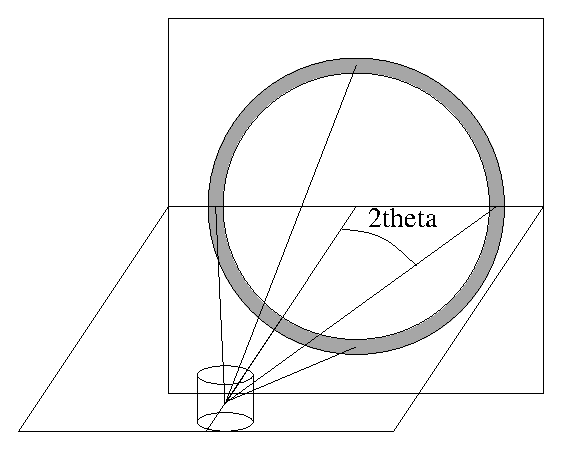
\includegraphics[width=0.6\textwidth]{figures/powder.eps}
  \end{center}
\caption{The scattering geometry of a powder sample showing part of the
Debye-Scherrer cone (solid lines) and the Debye-Scherrer circle (grey).}
\label{coneFig}
\end{figure}

Equation (\ref{Bragg}) may be cast into the form
\begin{equation}
|\boldsymbol{Q}| = 2 |\boldsymbol{k}| \sin \theta ,
\end{equation}
where \textbf{Q} is a vector of the reciprocal lattice, and \textbf{k} is
the wave vector of the x-ray. It is seen that only
reciprocal vectors fulfilling $|\boldsymbol{Q}| < 2 |\boldsymbol{k}|$
contribute to the scattering.
For a complete treatment of the powder sample, one needs to take
into account all these \textbf{Q}-values, since each of them contribute
to the attenuation.

The strength of the Bragg reflections is given by their structure factors
\begin{equation}
 \left| \sum_j b_j \exp(\boldsymbol{R}_j \cdot \boldsymbol{Q}) \right|^2 ,
\end{equation}
where the sum runs over all atoms in one unit cell. This structure factor is
non-zero only when $Q$ equals a reciprocal lattice vector.

The textbook expression for the scattering cross section
corresponding to one Debye-Scherrer cone reads \cite[ch.3.6]{squires}, with $V=N V_0$ being the total sample volume:
\begin{equation}
\sigma_\mathrm{cone}
  = \frac{V}{V_0^2} \frac{\lambda^3}{4 \sin \theta} \sum_Q |F(Q)|^2 .
\end{equation}
For our purpose, this expression should be changed slightly.
Firstly, the sum over structure factors for a particular $Q$ is replaced
by the sum over essentially different reflections multiplied by their
multiplicity, $j$. Then, a finite packing factor, $f$, is defined for the powder,
and finally, the Debye-Waller factor is multiplied on the elastic cross section
to take lattice vibrations into account (no inelastic background is simulated,
however). We then reach
\begin{eqnarray}
\sigma_\mathrm{cone, Q}
 & = & j_Q f \exp(-2W) \frac{V}{V_0^2} \frac{\lambda^3}{4 \sin \theta} |F(Q)|^2 \\
 & = & f \exp(-2W) \frac{N}{V_0} \frac{4\pi^3}{k^2} \frac{j_Q |F(Q)|^2}{Q}
\end{eqnarray}
in the thin sample approximation. For samples of finite thickness, the
beam is being attenuated by the attenuation coefficient
\begin{equation}
\label{e:attenu}
\mu_\mathrm{Q} = \sigma_\mathrm{cone,Q} / V .
\end{equation}
For calibration it may be useful to consider the total intensity
scattered into a detector of effective height $h$, covering only
one reflection \cite[ch.3.6]{squires}.
A cut though the Debye-Scherrer cone perpendicular to its axis
is a circle. At the distance $r$ from the sample, the radius of this
circle is $r \sin(2\theta)$. Thus, the detector (in a small angle
approximation) counts a fraction $h / (2 \pi r \sin(2 \theta))$
of the scattered x-rays, giving a resulting count intensity:
\begin{equation}
I = \Psi \sigma_\mathrm{cone,Q} \frac{h}{2 \pi r \sin(2\theta)} ,
\end{equation}
where $\Psi$ is the flux at the sample position.

For clarity we repeat the meaning and unit of the symbols:
%
\begin{quote}\begin{tabular}{ccl}
$\Psi$ & s$^{-1}$m$^{-2}$ & Incoming intensity of x-rays \\
$I$    & s$^{-1}$ & Detected intensity of x-rays \\
$h$    & m        & Height of detector \\
$r$    & m        & Distance from sample to detector \\
$f$    & 1        & Packing factor of the powder \\
$j$    & 1        & Multiplicity of the reflection \\
$V_0$  & m$^{3}$  & Volume of unit cell\\
$|F(\boldsymbol{Q})|^2$ & m$^2$  & Structure factor \\
$\exp(-2W)$ & 1  & Debye-Waller factor \\
$\mu_\mathrm{Q}$ & m$^{-1}$ & Linear attenuation factor due to scattering from
one powder line. \\
\end{tabular}\end{quote}
%
%Often, one defines the {\em scattering power} as
%\begin{equation}
%Q \equiv N^2 \frac{|F(\boldsymbol{Q})|^2 \lambda^3}{V \sin(2\theta)}
% = N_c^2 V \frac{\rho'}{\rho} \frac{|F(\boldsymbol{Q})|^2 \lambda^3}{\sin(2\theta)} ,
%\end{equation}
%where $N$ is the number of unit cells.

A powder sample will in general have several allowed reflections
$\boldsymbol{Q}_j$, which will all contribute to the attenuation.
These reflections will have different values of
$|F(\boldsymbol{Q}_j)|^2$ (and hence of $Q_j$), $j_j$, $\exp(-2W_j)$,
and $\theta_j$.
The total attenuation through the sample due to scattering is given by
$\mu^s = \mu_\mathrm{inc}^s + \sum_j \mu^s_j $,
where $\mu_\mathrm{inc}^s$ represents the incoherent scattering.

\subsection{Algorithm}
The algorithm of \textbf{PowderN} can be summarized as
\begin{itemize}
\item Check if the x-ray intersects the sample (otherwise ignore
the following).
\item Calculate the attenuation coefficients for scattering and absorption.
\item Perform Monte Carlo choices to determine the scattering position,
scattering type (coherent/incoherent), and the outgoing direction.
\item Perform the necessary weight factor transformation.
\end{itemize}

%\subsection{Calculating the weight factor}

%\component{Powder\_N}{System}{$radius$, $thickness$, $h$, $xwidth$, $yheight$, $zdepth$, $\sigma_\mathrm{abs}$,
%  $\sigma_\mathrm{inc}$, $Vc$, $f_\mathrm{pack}$, reflections, format, DW, concentic, and more}{}{}

The powder diffraction component \textbf{PowderN} models a powder sample
with background coming only from incoherent scattering and no
multiple scattering. At the users choice, a given percentage of the incoming
events may be transmitted (attenuated) to model the direct beam. The component can also
assume \emph{concentric} shape, i.e. be used for describing sample environment (cryostat,
sample container etc.). 

The description of the powder comes from a file in one of the standard output formats LAZY, FULLPROF, or CRYSTALLOGRAPHICA.

%A usage example of this component can be found in the \\
%\verb+x-ray site/Tutorial/templateDIFF+ instrument from the \verb+mcgui+.

\subsection{Files formats: powder structures}

Data files of type \verb'lau' and \verb'laz' in the \MCX distribution data directory are self-documented in their header. 
%A list of common powder definition files is available in Table \ref{t:powders-data} (page \pageref{t:powders-data}). They do not need any additional parameters to be used, as in the example:
\begin{verbatim}
  PowderN(<geometry parameters>, filename="Al.laz")
\end{verbatim}
Other column-based file formats may also be imported e.g. with parameters such as:
\begin{verbatim}
  format=Crystallographica
  format=Fullprof
  format={1,2,3,4,0,0,0,0}
\end{verbatim}
In the latter case, the indices define order of columns parameters
multiplicity, lattice spacing, $F^2$, Debye-Waller factor and intrinsic line width.

The column signification may as well explicitely be set in the data file header using any of the lines:
\begin{verbatim}
  #column_j     <index of the multiplicity 'j' column>
  #column_d     <index of the d-spacing 'd' column>
  #column_F2    <index of the squared str. factor '|F|^2' column [b]>
  #column_F     <index of the structure factor norm '|F|' column>
  #column_DW    <index of the Debye-Waller factor 'DW' column>
  #column_Dd    <index of the relative line width Delta_d/d 'Dd' column>
  #column_inv2d <index of the 1/2d=sin(theta)/lambda 'inv2d' column>
  #column_q     <index of the scattering wavevector 'q' column>
\end{verbatim}

Other component parameters may as well be specified in the data file
header with lines e.g.:
\begin{verbatim}
  #V_rho        <value of atom number density [at/Angs^3]>
  #Vc           <value of unit cell volume Vc [Angs^3]>
  #sigma_abs    <value of Absorption cross section [barns]>
  #sigma_inc    <value of Incoherent cross section [barns]>
  #Debye_Waller <value of Debye-Waller factor DW>
  #Delta_d/d    <value of Delta_d/d width for all lines>
  #density      <value of material density [g/cm^3]>
  #weight       <value of material molar weight [g/mol]>
  #nb_atoms     <value of number of atoms per unit cell>
\end{verbatim}

Further details on file formats are available in the \texttt{mxdoc} page
of the component.

\subsection{Geometry, physical properties, concentricity}
The sample has the shape of a solid cylinder, radius $r$ and height $h$ or a box-shaped
sample of size $xwidth$ x $yheight$ x $zdepth$. At the users choice, an inner 'hollow' can be
specified using the parameter $thickness$. 


%As the Isotropic\_Sqw component~\ref{s:isotropic-sqw}, 
PowderN can assume a \emph{concentric} shape, i.e.
can contain other components inside the inner hollow. To allow this, two almost identical copies
of the PowderN components must be set up \emph{around} the internal component(s), for example:


\begin{verbatim}
COMPONENT Cryo = PowderN(reflections="Al.laz", radius = 0.01, thickness = 0.001,
                          concentric = 1)
AT (0,0,0) RELATIVE Somewhere

COMPONENT Sample = some_other_component(with geometry FULLY enclosed in the hollow)
AT (0,0,0) RELATIVE Somewhere

COMPONENT Cryo2 = COPY(Cryo)(concentric = 0)
AT (0,0,0) RELATIVE Somewhere
\end{verbatim}

As outlined, the first instance of PowderN \emph{must} have \texttt{concentric = 1} and the second instance \emph{must}
have \texttt{concentric = 0}. Furthermore, the component(s) inside the hollow \emph{must} have a geometry which can
be fully contained inside the hollow.


In addition to the coherent scattering specified in the \verb+reflections+ file, absorption- and incoherent 
cross sections can be given using the input parameters $\sigma_c^a$ and $\sigma_i^s$.


The Bragg scattering from the powder,
$\sigma_c^s$ is calculated from the input file, with the parameters
$Q$, $|F(Q)|^2$, and $j$ for the scattering vector, structure factor, and
multiplicity, respectively. The volume of the unit cell is denoted $Vc$,
while the sample packing factor is $f_\mathrm{pack}$.


%Further, the incoherent scattering is only taken into account
%by the attenuation of the beam, given by (\ref{e:attenu})
%and $\sigma_c^a$.
%The incoherently scattered x-rays are not
%propagated through to the detector, but rather not generated at all.

Focusing is performed by only scattering into one angular
interval, $d\phi$ of the Debye-Scherrer circle. The center of this
interval is located at the point where the Debye-Scherrer circle
intersects the half-plane defined by the initial velocity, $\boldsymbol{v}_\mathrm{i}$,
and a user-specified vector, $\boldsymbol{f}$.

%The input parameters for this component are
%
%\begin{quote}\begin{tabular}{ccl}
%$r$ & m & Radius of cylinder \\
%$h$ & m & Height of cylinder \\
%$\sigma_c^a$ & fm$^2$ & Absorption cross section per unit cell (at 2200 m/s) \\
%$\sigma_{i,c}^s$ & (fm)$^2$ & Incoherent scattering cross section per unit cell \\
%$\rho'/\rho$ & 1 & Packing factor \\
%$V_c$ & \AA$^3$ & Volume of unit cell \\
%$\boldsymbol{Q}$ & \AA$^{-1}$ & The reciprocal lattice vector under consideration \\
%$|F(\textbf{Q}_j)|^2$ & (fm)$^2$ &
% Structure factor \\
%$j$ & 1 & Multiplicity of reflection \\
%$\exp(-2W)$ & 1 & Debye-Waller factor \\
%$d\phi$ & deg & Angular interval of focusing \\
%$f_x$ & m & \\
%$f_y$ & m & Focusing vector\\
%$f_z$ & m & \\
%\end{tabular}\end{quote}

\subsection{Powder scattering}
An ideal powder sample consists of many small
crystallites, although each crystallite is sufficiently
large not to cause measurable size broadening.
The orientation of the crystallites is evenly distributed,
and there is thus always a large number of
crystallites oriented to fulfill the Bragg condition
\begin{equation}   \label{Bragg}
n \lambda = 2 d \sin \theta ,
\end{equation}
where $n$ is the order of the scattering (an integer), $\lambda$
is the x-ray wavelength, $d$ is the lattice spacing of the sample,
and $2 \theta$ is the scattering angle, see figure \ref{coneFig}.
As all crystal orientations
are realised in a powder sample, the x-rays are scattered within a
{\em Debye-Scherrer cone} of opening angle $4 \theta$ \cite{bacon}.

\begin{figure}
  \begin{center}
    \psfrag{2theta}[c][c]{$2\theta$}
    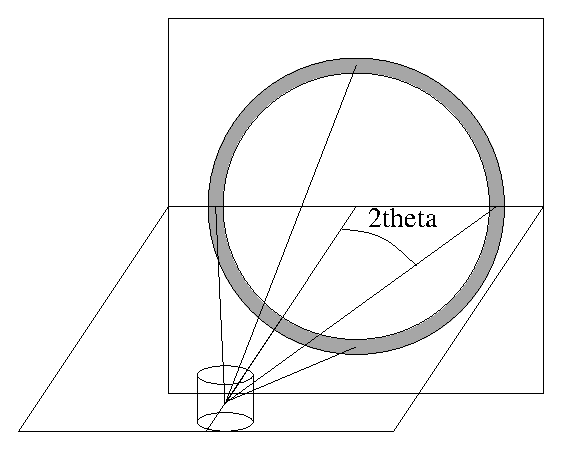
\includegraphics[width=0.6\textwidth]{figures/powder.eps}
  \end{center}
\caption{The scattering geometry of a powder sample showing part of the
Debye-Scherrer cone (solid lines) and the Debye-Scherrer circle (grey).}
\label{coneFig}
\end{figure}

Equation (\ref{Bragg}) may be cast into the form
\begin{equation}
|\boldsymbol{Q}| = 2 |\boldsymbol{k}| \sin \theta ,
\end{equation}
where \textbf{Q} is a vector of the reciprocal lattice, and \textbf{k} is
the wave vector of the x-ray. It is seen that only
reciprocal vectors fulfilling $|\boldsymbol{Q}| < 2 |\boldsymbol{k}|$
contribute to the scattering.
For a complete treatment of the powder sample, one needs to take
into account all these \textbf{Q}-values, since each of them contribute
to the attenuation.

The strength of the Bragg reflections is given by their structure factors
\begin{equation}
 \left| \sum_j b_j \exp(\boldsymbol{R}_j \cdot \boldsymbol{Q}) \right|^2 ,
\end{equation}
where the sum runs over all atoms in one unit cell. This structure factor is
non-zero only when $Q$ equals a reciprocal lattice vector.

The textbook expression for the scattering cross section
corresponding to one Debye-Scherrer cone reads \cite[ch.3.6]{squires}, with $V=N V_0$ being the total sample volume:
\begin{equation}
\sigma_\mathrm{cone}
  = \frac{V}{V_0^2} \frac{\lambda^3}{4 \sin \theta} \sum_Q |F(Q)|^2 .
\end{equation}
For our purpose, this expression should be changed slightly.
Firstly, the sum over structure factors for a particular $Q$ is replaced
by the sum over essentially different reflections multiplied by their
multiplicity, $j$. Then, a finite packing factor, $f$, is defined for the powder,
and finally, the Debye-Waller factor is multiplied on the elastic cross section
to take lattice vibrations into account (no inelastic background is simulated,
however). We then reach
\begin{eqnarray}
\sigma_\mathrm{cone, Q}
 & = & j_Q f \exp(-2W) \frac{V}{V_0^2} \frac{\lambda^3}{4 \sin \theta} |F(Q)|^2 \\
 & = & f \exp(-2W) \frac{N}{V_0} \frac{4\pi^3}{k^2} \frac{j_Q |F(Q)|^2}{Q}
\end{eqnarray}
in the thin sample approximation. For samples of finite thickness, the
beam is being attenuated by the attenuation coefficient
\begin{equation}
\label{e:attenu}
\mu_\mathrm{Q} = \sigma_\mathrm{cone,Q} / V .
\end{equation}
For calibration it may be useful to consider the total intensity
scattered into a detector of effective height $h$, covering only
one reflection \cite[ch.3.6]{squires}.
A cut though the Debye-Scherrer cone perpendicular to its axis
is a circle. At the distance $r$ from the sample, the radius of this
circle is $r \sin(2\theta)$. Thus, the detector (in a small angle
approximation) counts a fraction $h / (2 \pi r \sin(2 \theta))$
of the scattered x-rays, giving a resulting count intensity:
\begin{equation}
I = \Psi \sigma_\mathrm{cone,Q} \frac{h}{2 \pi r \sin(2\theta)} ,
\end{equation}
where $\Psi$ is the flux at the sample position.

For clarity we repeat the meaning and unit of the symbols:
%
\begin{quote}\begin{tabular}{ccl}
$\Psi$ & s$^{-1}$m$^{-2}$ & Incoming intensity of x-rays \\
$I$    & s$^{-1}$ & Detected intensity of x-rays \\
$h$    & m        & Height of detector \\
$r$    & m        & Distance from sample to detector \\
$f$    & 1        & Packing factor of the powder \\
$j$    & 1        & Multiplicity of the reflection \\
$V_0$  & m$^{3}$  & Volume of unit cell\\
$|F(\boldsymbol{Q})|^2$ & m$^2$  & Structure factor \\
$\exp(-2W)$ & 1  & Debye-Waller factor \\
$\mu_\mathrm{Q}$ & m$^{-1}$ & Linear attenuation factor due to scattering from
one powder line. \\
\end{tabular}\end{quote}
%
%Often, one defines the {\em scattering power} as
%\begin{equation}
%Q \equiv N^2 \frac{|F(\boldsymbol{Q})|^2 \lambda^3}{V \sin(2\theta)}
% = N_c^2 V \frac{\rho'}{\rho} \frac{|F(\boldsymbol{Q})|^2 \lambda^3}{\sin(2\theta)} ,
%\end{equation}
%where $N$ is the number of unit cells.

A powder sample will in general have several allowed reflections
$\boldsymbol{Q}_j$, which will all contribute to the attenuation.
These reflections will have different values of
$|F(\boldsymbol{Q}_j)|^2$ (and hence of $Q_j$), $j_j$, $\exp(-2W_j)$,
and $\theta_j$.
The total attenuation through the sample due to scattering is given by
$\mu^s = \mu_\mathrm{inc}^s + \sum_j \mu^s_j $,
where $\mu_\mathrm{inc}^s$ represents the incoherent scattering.

\subsection{Algorithm}
The algorithm of \textbf{PowderN} can be summarized as
\begin{itemize}
\item Check if the x-ray intersects the sample (otherwise ignore
the following).
\item Calculate the attenuation coefficients for scattering and absorption.
\item Perform Monte Carlo choices to determine the scattering position,
scattering type (coherent/incoherent), and the outgoing direction.
\item Perform the necessary weight factor transformation.
\end{itemize}

%\subsection{Calculating the weight factor}

%\component{Powder\_N}{System}{$radius$, $thickness$, $h$, $xwidth$, $yheight$, $zdepth$, $\sigma_\mathrm{abs}$,
%  $\sigma_\mathrm{inc}$, $Vc$, $f_\mathrm{pack}$, reflections, format, DW, concentic, and more}{}{}

The powder diffraction component \textbf{PowderN} models a powder sample
with background coming only from incoherent scattering and no
multiple scattering. At the users choice, a given percentage of the incoming
events may be transmitted (attenuated) to model the direct beam. The component can also
assume \emph{concentric} shape, i.e. be used for describing sample environment (cryostat,
sample container etc.). 

The description of the powder comes from a file in one of the standard output formats LAZY, FULLPROF, or CRYSTALLOGRAPHICA.

%A usage example of this component can be found in the \\
%\verb+x-ray site/Tutorial/templateDIFF+ instrument from the \verb+mcgui+.

\subsection{Files formats: powder structures}

Data files of type \verb'lau' and \verb'laz' in the \MCX distribution data directory are self-documented in their header. 
%A list of common powder definition files is available in Table \ref{t:powders-data} (page \pageref{t:powders-data}). They do not need any additional parameters to be used, as in the example:
\begin{verbatim}
  PowderN(<geometry parameters>, filename="Al.laz")
\end{verbatim}
Other column-based file formats may also be imported e.g. with parameters such as:
\begin{verbatim}
  format=Crystallographica
  format=Fullprof
  format={1,2,3,4,0,0,0,0}
\end{verbatim}
In the latter case, the indices define order of columns parameters
multiplicity, lattice spacing, $F^2$, Debye-Waller factor and intrinsic line width.

The column signification may as well explicitely be set in the data file header using any of the lines:
\begin{verbatim}
  #column_j     <index of the multiplicity 'j' column>
  #column_d     <index of the d-spacing 'd' column>
  #column_F2    <index of the squared str. factor '|F|^2' column [b]>
  #column_F     <index of the structure factor norm '|F|' column>
  #column_DW    <index of the Debye-Waller factor 'DW' column>
  #column_Dd    <index of the relative line width Delta_d/d 'Dd' column>
  #column_inv2d <index of the 1/2d=sin(theta)/lambda 'inv2d' column>
  #column_q     <index of the scattering wavevector 'q' column>
\end{verbatim}

Other component parameters may as well be specified in the data file
header with lines e.g.:
\begin{verbatim}
  #V_rho        <value of atom number density [at/Angs^3]>
  #Vc           <value of unit cell volume Vc [Angs^3]>
  #sigma_abs    <value of Absorption cross section [barns]>
  #sigma_inc    <value of Incoherent cross section [barns]>
  #Debye_Waller <value of Debye-Waller factor DW>
  #Delta_d/d    <value of Delta_d/d width for all lines>
  #density      <value of material density [g/cm^3]>
  #weight       <value of material molar weight [g/mol]>
  #nb_atoms     <value of number of atoms per unit cell>
\end{verbatim}

Further details on file formats are available in the \texttt{mxdoc} page
of the component.

\subsection{Geometry, physical properties, concentricity}
The sample has the shape of a solid cylinder, radius $r$ and height $h$ or a box-shaped
sample of size $xwidth$ x $yheight$ x $zdepth$. At the users choice, an inner 'hollow' can be
specified using the parameter $thickness$. 


%As the Isotropic\_Sqw component~\ref{s:isotropic-sqw}, 
PowderN can assume a \emph{concentric} shape, i.e.
can contain other components inside the inner hollow. To allow this, two almost identical copies
of the PowderN components must be set up \emph{around} the internal component(s), for example:


\begin{verbatim}
COMPONENT Cryo = PowderN(reflections="Al.laz", radius = 0.01, thickness = 0.001,
                          concentric = 1)
AT (0,0,0) RELATIVE Somewhere

COMPONENT Sample = some_other_component(with geometry FULLY enclosed in the hollow)
AT (0,0,0) RELATIVE Somewhere

COMPONENT Cryo2 = COPY(Cryo)(concentric = 0)
AT (0,0,0) RELATIVE Somewhere
\end{verbatim}

As outlined, the first instance of PowderN \emph{must} have \texttt{concentric = 1} and the second instance \emph{must}
have \texttt{concentric = 0}. Furthermore, the component(s) inside the hollow \emph{must} have a geometry which can
be fully contained inside the hollow.


In addition to the coherent scattering specified in the \verb+reflections+ file, absorption- and incoherent 
cross sections can be given using the input parameters $\sigma_c^a$ and $\sigma_i^s$.


The Bragg scattering from the powder,
$\sigma_c^s$ is calculated from the input file, with the parameters
$Q$, $|F(Q)|^2$, and $j$ for the scattering vector, structure factor, and
multiplicity, respectively. The volume of the unit cell is denoted $Vc$,
while the sample packing factor is $f_\mathrm{pack}$.


%Further, the incoherent scattering is only taken into account
%by the attenuation of the beam, given by (\ref{e:attenu})
%and $\sigma_c^a$.
%The incoherently scattered x-rays are not
%propagated through to the detector, but rather not generated at all.

Focusing is performed by only scattering into one angular
interval, $d\phi$ of the Debye-Scherrer circle. The center of this
interval is located at the point where the Debye-Scherrer circle
intersects the half-plane defined by the initial velocity, $\boldsymbol{v}_\mathrm{i}$,
and a user-specified vector, $\boldsymbol{f}$.

%The input parameters for this component are
%
%\begin{quote}\begin{tabular}{ccl}
%$r$ & m & Radius of cylinder \\
%$h$ & m & Height of cylinder \\
%$\sigma_c^a$ & fm$^2$ & Absorption cross section per unit cell (at 2200 m/s) \\
%$\sigma_{i,c}^s$ & (fm)$^2$ & Incoherent scattering cross section per unit cell \\
%$\rho'/\rho$ & 1 & Packing factor \\
%$V_c$ & \AA$^3$ & Volume of unit cell \\
%$\boldsymbol{Q}$ & \AA$^{-1}$ & The reciprocal lattice vector under consideration \\
%$|F(\textbf{Q}_j)|^2$ & (fm)$^2$ &
% Structure factor \\
%$j$ & 1 & Multiplicity of reflection \\
%$\exp(-2W)$ & 1 & Debye-Waller factor \\
%$d\phi$ & deg & Angular interval of focusing \\
%$f_x$ & m & \\
%$f_y$ & m & Focusing vector\\
%$f_z$ & m & \\
%\end{tabular}\end{quote}

\subsection{Powder scattering}
An ideal powder sample consists of many small
crystallites, although each crystallite is sufficiently
large not to cause measurable size broadening.
The orientation of the crystallites is evenly distributed,
and there is thus always a large number of
crystallites oriented to fulfill the Bragg condition
\begin{equation}   \label{Bragg}
n \lambda = 2 d \sin \theta ,
\end{equation}
where $n$ is the order of the scattering (an integer), $\lambda$
is the x-ray wavelength, $d$ is the lattice spacing of the sample,
and $2 \theta$ is the scattering angle, see figure \ref{coneFig}.
As all crystal orientations
are realised in a powder sample, the x-rays are scattered within a
{\em Debye-Scherrer cone} of opening angle $4 \theta$ \cite{bacon}.

\begin{figure}
  \begin{center}
    \psfrag{2theta}[c][c]{$2\theta$}
    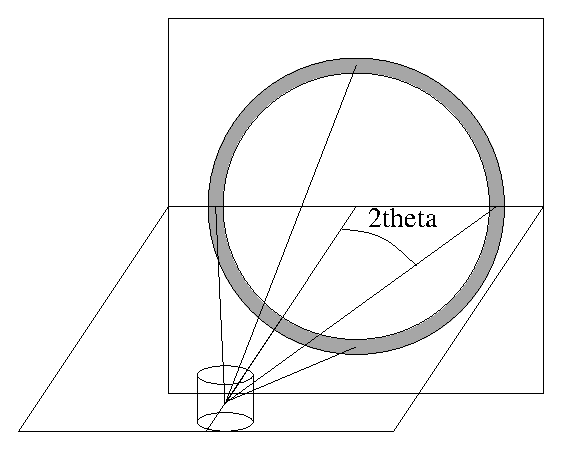
\includegraphics[width=0.6\textwidth]{figures/powder.eps}
  \end{center}
\caption{The scattering geometry of a powder sample showing part of the
Debye-Scherrer cone (solid lines) and the Debye-Scherrer circle (grey).}
\label{coneFig}
\end{figure}

Equation (\ref{Bragg}) may be cast into the form
\begin{equation}
|\boldsymbol{Q}| = 2 |\boldsymbol{k}| \sin \theta ,
\end{equation}
where \textbf{Q} is a vector of the reciprocal lattice, and \textbf{k} is
the wave vector of the x-ray. It is seen that only
reciprocal vectors fulfilling $|\boldsymbol{Q}| < 2 |\boldsymbol{k}|$
contribute to the scattering.
For a complete treatment of the powder sample, one needs to take
into account all these \textbf{Q}-values, since each of them contribute
to the attenuation.

The strength of the Bragg reflections is given by their structure factors
\begin{equation}
 \left| \sum_j b_j \exp(\boldsymbol{R}_j \cdot \boldsymbol{Q}) \right|^2 ,
\end{equation}
where the sum runs over all atoms in one unit cell. This structure factor is
non-zero only when $Q$ equals a reciprocal lattice vector.

The textbook expression for the scattering cross section
corresponding to one Debye-Scherrer cone reads \cite[ch.3.6]{squires}, with $V=N V_0$ being the total sample volume:
\begin{equation}
\sigma_\mathrm{cone}
  = \frac{V}{V_0^2} \frac{\lambda^3}{4 \sin \theta} \sum_Q |F(Q)|^2 .
\end{equation}
For our purpose, this expression should be changed slightly.
Firstly, the sum over structure factors for a particular $Q$ is replaced
by the sum over essentially different reflections multiplied by their
multiplicity, $j$. Then, a finite packing factor, $f$, is defined for the powder,
and finally, the Debye-Waller factor is multiplied on the elastic cross section
to take lattice vibrations into account (no inelastic background is simulated,
however). We then reach
\begin{eqnarray}
\sigma_\mathrm{cone, Q}
 & = & j_Q f \exp(-2W) \frac{V}{V_0^2} \frac{\lambda^3}{4 \sin \theta} |F(Q)|^2 \\
 & = & f \exp(-2W) \frac{N}{V_0} \frac{4\pi^3}{k^2} \frac{j_Q |F(Q)|^2}{Q}
\end{eqnarray}
in the thin sample approximation. For samples of finite thickness, the
beam is being attenuated by the attenuation coefficient
\begin{equation}
\label{e:attenu}
\mu_\mathrm{Q} = \sigma_\mathrm{cone,Q} / V .
\end{equation}
For calibration it may be useful to consider the total intensity
scattered into a detector of effective height $h$, covering only
one reflection \cite[ch.3.6]{squires}.
A cut though the Debye-Scherrer cone perpendicular to its axis
is a circle. At the distance $r$ from the sample, the radius of this
circle is $r \sin(2\theta)$. Thus, the detector (in a small angle
approximation) counts a fraction $h / (2 \pi r \sin(2 \theta))$
of the scattered x-rays, giving a resulting count intensity:
\begin{equation}
I = \Psi \sigma_\mathrm{cone,Q} \frac{h}{2 \pi r \sin(2\theta)} ,
\end{equation}
where $\Psi$ is the flux at the sample position.

For clarity we repeat the meaning and unit of the symbols:
%
\begin{quote}\begin{tabular}{ccl}
$\Psi$ & s$^{-1}$m$^{-2}$ & Incoming intensity of x-rays \\
$I$    & s$^{-1}$ & Detected intensity of x-rays \\
$h$    & m        & Height of detector \\
$r$    & m        & Distance from sample to detector \\
$f$    & 1        & Packing factor of the powder \\
$j$    & 1        & Multiplicity of the reflection \\
$V_0$  & m$^{3}$  & Volume of unit cell\\
$|F(\boldsymbol{Q})|^2$ & m$^2$  & Structure factor \\
$\exp(-2W)$ & 1  & Debye-Waller factor \\
$\mu_\mathrm{Q}$ & m$^{-1}$ & Linear attenuation factor due to scattering from
one powder line. \\
\end{tabular}\end{quote}
%
%Often, one defines the {\em scattering power} as
%\begin{equation}
%Q \equiv N^2 \frac{|F(\boldsymbol{Q})|^2 \lambda^3}{V \sin(2\theta)}
% = N_c^2 V \frac{\rho'}{\rho} \frac{|F(\boldsymbol{Q})|^2 \lambda^3}{\sin(2\theta)} ,
%\end{equation}
%where $N$ is the number of unit cells.

A powder sample will in general have several allowed reflections
$\boldsymbol{Q}_j$, which will all contribute to the attenuation.
These reflections will have different values of
$|F(\boldsymbol{Q}_j)|^2$ (and hence of $Q_j$), $j_j$, $\exp(-2W_j)$,
and $\theta_j$.
The total attenuation through the sample due to scattering is given by
$\mu^s = \mu_\mathrm{inc}^s + \sum_j \mu^s_j $,
where $\mu_\mathrm{inc}^s$ represents the incoherent scattering.

\subsection{Algorithm}
The algorithm of \textbf{PowderN} can be summarized as
\begin{itemize}
\item Check if the x-ray intersects the sample (otherwise ignore
the following).
\item Calculate the attenuation coefficients for scattering and absorption.
\item Perform Monte Carlo choices to determine the scattering position,
scattering type (coherent/incoherent), and the outgoing direction.
\item Perform the necessary weight factor transformation.
\end{itemize}

%\subsection{Calculating the weight factor}
          \newpage
\section{Perfect\_crystal: A Darwin-width domniated single crystal model}

\index{Samples!single crystal, darwin}
\label{perfect_crystal}
\mcdoccomp{samples/Perfect_crystal.parms}

Pedning Further Documetation
\newpage
\section{Single\_crystal: The single crystal component}
\label{s:Single_crystal}
\index{Samples!Single crystal diffraction}
\index{Diffraction}
\index{Incoherent elastic scattering}
\index{Multiple scattering}

%\component{Single\_crystal}{Kristian Nielsen}{$x_{width}, y_{height}, z_{thick}$,$\vec a, \vec b, \vec c, \Delta d/d$, mosaic, reflections}{$\sigma_{abs}, \sigma_{inc}$, ...}{Partially validated, centered. Further validation undergoing. Known BUGS: The component is known not to work as a Bragg monochromator, likely the problem relates to the internal definition of the reciprocal space. Possibly related to this, the model of anistropic mosaic is broken - always use a non-zero isotropic mosaic. Also, always use a non-zero value of the $\Delta d/d$ parameter.}
\mcdoccomp{samples/Single_crystal.parms}

The \textbf{Single\_crystal} component models a thick, flat single crystal
with multiple scattering and absorption with elastic coherent scattering.
An elastic incoherent background may also be simulated.
It may be used to describe samples for diffraction,
but also for accurate monochromator descriptions.
The component is currently under further review. The current documentation is outdated, especially with respect to the model of crystal mosaicity.

The input parameters for the component are \textit{xwidth},
\textit{yheight}, and \textit{zdepth} to define the dimensions of the
crystal in meters (area is centered); \textit{delta\_d\_d} to give the
value of $\Delta d/d$ (no unit);
$(\textit{ax}, \textit{ay}, \textit{az})$, $(\textit{bx}, \textit{by},
\textit{bz})$, and $(\textit{cx}, \textit{cy}, \textit{cz})$ to define
the axes of the direct lattice of the crystal (the sides of the unit
cell) in units of {\AA}ngstr{\o}m; and \textit{reflections}, a string
giving the name of the file with the list of structure factors to
consider.
The mosaic is specified \emph{either} isotropically as
\textit{mosaic}, \emph{or} anisotropically as \textit{mosaic\_h}
(rotation around the $Y$ axis), \textit{mosaic\_v} (rotation around the
$Z$ axis), and \textit{mosaic\_n} (rotation around the $X$ axis); in all
cases in units of full-width-half-maximum minutes of arc.

Optionally, the absorption cross-section at 2200 m/s and the incoherent
cross-section may be given as \textit{absorption} and
\textit{incoherent} (in barns), with default of zero; and
\textit{p\_transmit} may be assigned a fixed Monte Carlo probability for
transmission through the crystal without any interaction.

The user must specify a list of reciprocal lattice vectors
$\boldsymbol{\tau}$ to consider along with their structure factors
$|F_{\boldsymbol{\tau}}|^2$. The user must also specify the coordinates
(in direct space) of the unit cell axes $\boldsymbol{a}$,
$\boldsymbol{b}$, and $\boldsymbol{c}$, from which the reciprocal lattice
will be computed. See section \ref{s:Single_crystal_implement} for file format specifications.

In addition to coherent scattering, \textbf{Single\_crystal} also
handles incoherent scattering and absorption. The incoherent scattering
cross-section is supplied by the user as a constant
$\sigma_\textrm{inc}$. The absorption cross-section is supplied by the user at
2200~m/s, so the actual cross-section for a neutron of velocity $v$ is
$\sigma_\textrm{abs} = \sigma_{2200} \frac{\textrm{2200~m/s}}{v}$.

\subsection{The physical model}

The textbook expression for the scattering cross-section of a crystal
is~\cite[ch.3]{squires}:
\begin{equation}
\label{eq:sigma_coh_el}
\left(\frac{d\sigma}{d\Omega}\right)_\textrm{coh.el.} =
        N\frac{(2\pi)^3}{V_0}\sum_{\boldsymbol{\tau}}
        \delta(\boldsymbol{\tau} - \boldsymbol{\kappa})|F_{\boldsymbol{\tau}}|^2
\end{equation}
Here $|F_{\boldsymbol{\tau}}|^2$ is the structure factor
(defined in section~\ref{powder}), $N$ is the
number of unit cells, $V_0$ is the volume of an
individual unit cell, and $\boldsymbol{\kappa} (= \textbf{k}_i - \textbf{k}_f)$
is the scattering vector. $\delta(\boldsymbol{x})$ is a 3-dimensional delta
function in reciprocal space,
so for given incoming wave vector $\textbf{k}_i$ and lattice vector
${\boldsymbol{\tau}}$, only a single final wave vector $\textbf{k}_f$ is allowed.
In general, this wavevector will not fulfill the conditions for elastic
scattering $(k_f = k_i)$.
In a real crystal, however, reflections are not perfectly sharp. Because
of imperfection and finite-size effects, there will be a small region
around $\boldsymbol{\tau}$ in reciprocal space of possible scattering vectors.

\textbf{Single\_crystal} simulates a crystal with a mosaic spread
$\eta$ and a lattice plane spacing uncertainty $\Delta d/d$. In such
crystals the reflections will not be completely sharp;
there will be a small region around each reciprocal lattice point of the
crystal that contains valid scattering vectors.

We model the mosaicity and $\Delta d/d$ of the crystal with
3-dimensional Gaussian functions in reciprocal space (see
figure~\ref{fig:crystal-reciprocal-space}). Two of the axes of the
Gaussian are perpendicular to the reciprocal lattice vector $\boldsymbol{\tau}$ and model
the mosaicity. The third one is parallel to $\boldsymbol{\tau}$ and models
$\Delta d/d$. We assume that the
mosaicity is small so that the possible directions of the scattering
vector may be approximated with a Gaussian in rectangular
coordinates.
\begin{figure}[t]
  \begin{center}
    \psfrag{ki}[r][r]{$\boldsymbol{k}_\textrm{i}$}
    \psfrag{kf}[l][l]{$\boldsymbol{k}_\textrm{f}$}
    \psfrag{tau}[r][r]{$\boldsymbol{\tau}$}
    \psfrag{mosaic}[l][l]{$\eta$}
    \psfrag{del-d-d}[l][l]{$\Delta d/d$}
    \psfrag{Ewald}[l][l]{Ewald}
    \psfrag{Sphere}[l][l]{Sphere}
    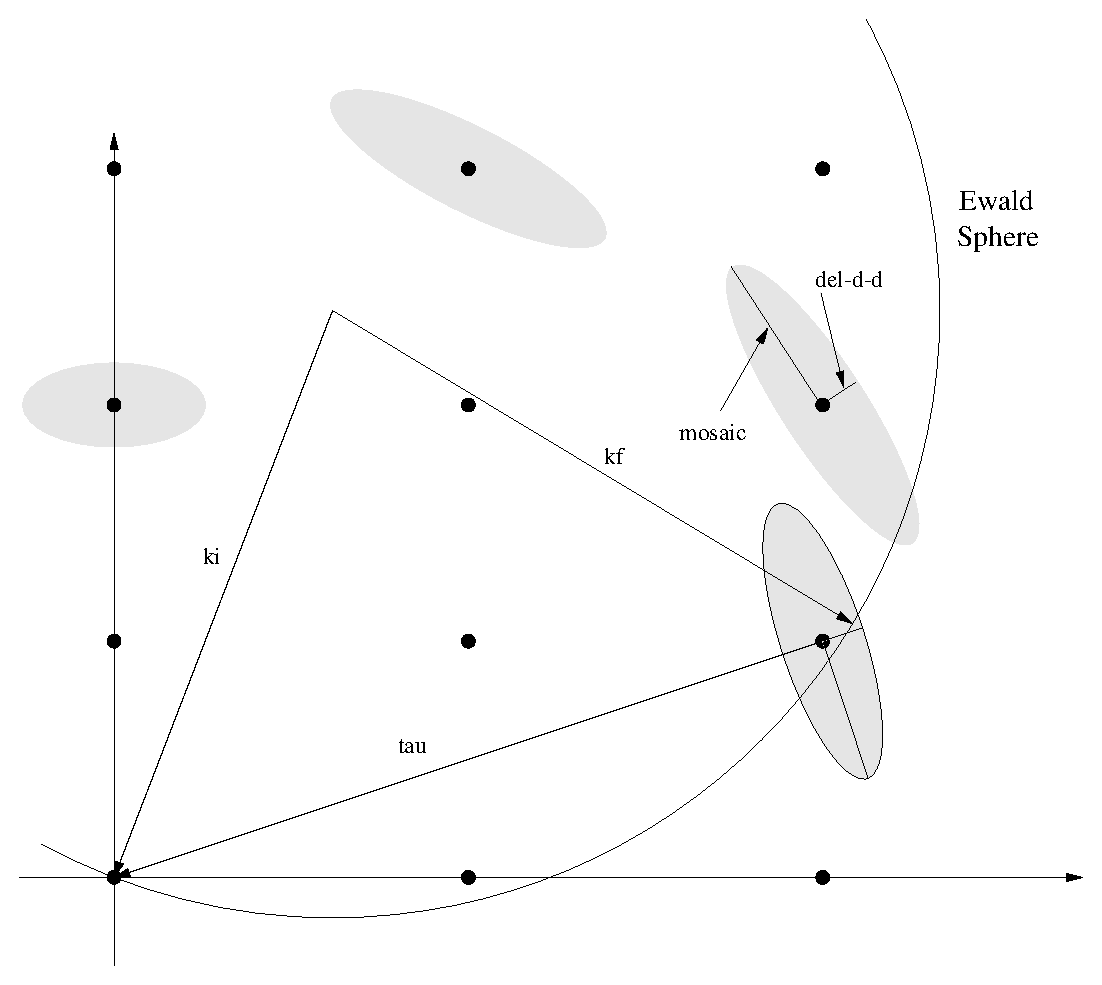
\includegraphics[width=0.7\textwidth]{figures/recip_space3}
  \end{center}
\caption{Ewald sphere construction for a single neutron showing the
    Gaussian broadening of reciprocal lattice points in their local
    coordinate system.}
\label{fig:crystal-reciprocal-space}
\end{figure}

If the mosaic is isotropic (the same in all directions), the two
Gaussian axes perpendicular to $\boldsymbol{\tau}$ are simply arbitrary
normal vectors of equal length given by the mosaic. But if the mosaic
is anisotropic, the two perpendicular axes will in general be different
for each scattering vector. In the absence of anything better,
\textbf{Single\_crystal} uses a model which is at least mathematically
plausible and which works as expected in the two common cases:
(1)~isotropic mosaic, and (2)~two mosaic directions (``horizontal and
vertical mosaic'') perpendicular to a scattering vector.

The basis for the model is a three-dimensional Gaussian distribution in
Euler angles giving the orientation probability distribution for the
micro-crystals; that is, the misorientation is given by small rotations
around the $X$, $Y$, and $Z$ axes, with the rotation angles having (in
general different) Gaussian probability distributions. For given
scattering vector $\boldsymbol{\tau}$, a rotation of the micro-crystals
around an axis parallel to $\boldsymbol{\tau}$ has no effect on the
direction of the scattering vector. Suppose we form the intersection
between the three-dimensional Gaussian in Euler angles and a plane
through the origin perpendicular to $\boldsymbol{\tau}$. This gives a
two-dimensional Gaussian, say with axes defined by unit vectors
$\boldsymbol{g}_1$ and $\boldsymbol{g}_2$ and mosaic widths $\eta_1$ and
$\eta_2$.

We now let the mosaic for $\boldsymbol{\tau}$ be defined by rotations
around $\boldsymbol{g}_1$ and $\boldsymbol{g}_2$ with angles having
Gaussian distributions of widths $\eta_1$ and $\eta_2$. Since
$\boldsymbol{g}_1$, $\boldsymbol{g}_2$, and $\boldsymbol{\tau}$ are
perpendicular, a small rotation of $\boldsymbol{\tau}$ around
$\boldsymbol{g}_1$ will change $\boldsymbol{\tau}$ in the direction of
$\boldsymbol{g}_2$. The two axes of the Gaussian mosaic in reciprocal
space that are perpendicular to $\boldsymbol{\tau}$ will thus be given
by $\tau\eta_2\boldsymbol{g}_1$ and $\tau\eta_1\boldsymbol{g}_2$.

We now derive a quantitative expression for the scattering cross-section
of the crystal in the model. For this, we introduce a \emph{local
  coordinate system} for each reciprocal lattice point
$\boldsymbol{\tau}$ and use $\boldsymbol{x}$ for vectors written in local
coordinates. The origin is $\boldsymbol{\tau}$, the first axis
is parallel to $\boldsymbol{\tau}$ and the other two axes are
perpendicular to $\boldsymbol{\tau}$. In the local coordinate system,
the 3-dimensional Gaussian is given by
\begin{equation}
  \label{eq:crystal-gauss-1}
  G(x_1,x_2,x_3) = \frac{1}{(\sqrt{2\pi})^3}\frac{1}{\sigma_1\sigma_2\sigma_3}
  e^{-\frac{1}{2}(\frac{x_1^2}{\sigma_1^2} +
  \frac{x_2^2}{\sigma_2^2} + \frac{x_3^2}{\sigma_3^2})}
\end{equation}
The axes of the Gaussian are $\sigma_1 = \tau\Delta d/d$ and $\sigma_2 =
\sigma_3 = \eta\tau$. Here we used the assumption that $\eta$ is small,
so that $\tan\eta \approx \eta$ (with $\eta$ given in radians).  By
introducing the diagonal matrix
$$
D = \left(
  \begin{array}[c]{ccc}
    \frac{1}{2}\sigma_1^2 & 0 & 0 \\
    0 & \frac{1}{2}\sigma_2^2 & 0 \\
    0 & 0 & \frac{1}{2}\sigma_3^2
  \end{array}\right)
$$
equation~(\ref{eq:crystal-gauss-1}) can be written as
\begin{equation}
  G(\boldsymbol{x}) =
  \frac{1}{(\sqrt{2\pi})^3}\frac{1}{\sigma_1\sigma_2\sigma_3}
  e^{-\boldsymbol{x}^\textrm{T} D \boldsymbol{x}}
\end{equation}
again with $\boldsymbol{x}=(x_1,x_2,x_3)$ written in local coordinates.

To get an expression in the coordinates of the reciprocal lattice of the
crystal, we introduce a matrix $U$ such that if $\boldsymbol{y} =
(y_1,y_2,y_3)$ are the global coordinates of a point in the crystal
reciprocal lattice, then $U(\boldsymbol{y} + \boldsymbol{\tau})$ are the
coordinates in the local coordinate system for $\boldsymbol{\tau}$. The
matrix $U$ is given by
$$ U^\textrm{T} = (\hat{u}_1, \hat{u}_2, \hat{u}_3), $$
where $\hat{u}_1$, $\hat{u}_2$, and $\hat{u}_3$ are the axes of the
local coordinate system, written in the global coordinates of the
reciprocal lattice. Thus
$\hat{u}_1 = \boldsymbol{\tau}/\tau$,  and $\hat{u}_2$ and $\hat{u}_3$ are
unit vectors perpendicular to $\hat{u}_1$ and to each other.
The matrix $U$ is unitarian, that is
$U^{-1} = U^\textrm{T}$. The translation between global and local
coordinates is
$$ \boldsymbol{x} = U(\boldsymbol{y} + \boldsymbol{\tau}) \qquad
   \boldsymbol{y} = U^\textrm{T} \boldsymbol{x} - \boldsymbol{\tau} $$

The expression for the 3-dimensional Gaussian in global coordinates is
\begin{equation}
  G(\boldsymbol{y}) =
  \frac{1}{(\sqrt{2\pi})^3}\frac{1}{\sigma_1\sigma_2\sigma_3}
  e^{-(U(\boldsymbol{y}+\boldsymbol{\tau}))^\textrm{T} D (U(\boldsymbol{y}+\boldsymbol{\tau}))}
\end{equation}
The elastic coherent cross-section is then given by
\begin{equation}
  \label{eq:crystal-cross-section}
  \left(\frac{d\sigma}{d\Omega}\right)_\textrm{coh.el.} =
        N\frac{(2\pi)^3}{V_0}\sum_{\boldsymbol{\tau}}
        G(\boldsymbol{\tau} - \boldsymbol{\kappa})
         |F_{\boldsymbol{\tau}}|^2
\end{equation}

\subsection{The algorithm}

The overview of the algorithm used in the Single\_crystal component is
as follows:
\begin{enumerate}
\item\label{enum:crystal-1} Check if the neutron intersects the
  crystal. If not, no action is taken.
\item\label{enum:crystal-2} Search through a list of reciprocal lattice
  points of interest, selecting those that are close enough to the Ewald
  sphere to have a non-vanishing scattering probability. From these,
  compute the total coherent cross-section $\sigma_\textrm{coh}$ (see
  below), the absorption cross-section $\sigma_\textrm{abs} = \sigma_\textrm{
  2200} \frac{\textrm{2200~m/s}}{v}$, and the total cross-section
  $\sigma_\textrm{tot} = \sigma_\textrm{coh}+\sigma_\textrm{inc}+\sigma_\textrm{abs}$.
\item\label{enum:crystal-3} The transmission probability is
  $\exp(- \frac{\sigma_\textrm{tot}}{V_0}\ell)$ where $\ell$ is the length of
  the flight path through the crystal. A Monte Carlo choice is
  performed to determine
  whether the neutron is transmitted. Optionally, the user may
  set a fixed Monte Carlo probability for the first scattering event,
  for example to boost the statistics for a weak reflection.
\item\label{enum:crystal-4} For non-transmission, the position at which
  the neutron will interact is selected from an exponential
  distribution. A Monte Carlo choice is made of whether to scatter
  coherently or incoherently. Absorption is treated by weight adjustment
  (see below).
\item\label{enum:crystal-5} For incoherent scattering, the outgoing wave
  vector $\boldsymbol{k}_\textrm{f}$ is selected with a random direction.
\item\label{enum:crystal-6} For coherent scattering, a reciprocal
  lattice vector is selected by a Monte Carlo choice, and
  $\boldsymbol{k}_\textrm{f}$ is found (see below).
\item\label{enum:crystal-7} Adjust the neutron weight as dictated by the
  Monte Carlo choices made.
\item\label{enum:crystal-8} Repeat from~(\ref{enum:crystal-2}) until the
  neutron is transmitted (to simulate multiple scattering).
\end{enumerate}

For point~\ref{enum:crystal-2}, the distance
\textit{dist} between a reciprocal lattice point and the Ewald sphere is
considered small enough to allow scattering if it is less than five
times the maximum axis of the Gaussian, $\textit{dist} \leq
5\max(\sigma_1,\sigma_2,\sigma_3)$.

\subsection{Choosing the outgoing wave vector}

The final wave vector $\boldsymbol{k}_\textrm{f}$ must lie on the
intersection between the Ewald sphere and the Gaussian ellipsoid. Since
$\eta$ and $\Delta d/d$ are assumed small, the intersection can be
approximated with a plane tangential to the sphere, see
figure~\ref{fig:crystal-scattering-tri}. The tangential point is taken
to lie on the line between the center of the Ewald sphere
$-\boldsymbol{k}_\textrm{i}$ and the reciprocal lattice point
$\boldsymbol{\tau}$. Since the radius of the Ewald sphere is $k_\textrm{
  i}$, this point is
$$ \boldsymbol{o}=(k_\textrm{i}/\rho - 1)\boldsymbol{\rho} - \boldsymbol{\tau} $$
where $\boldsymbol{\rho} = \boldsymbol{k}_\textrm{i} - \boldsymbol{\tau}$.
\begin{figure}[t]
  \begin{center}
    \psfrag{ki}[r][r]{$\boldsymbol{k}_\textrm{i}$}
    \psfrag{kf}[l][l]{$\boldsymbol{k}_\textrm{f}$}
    \psfrag{rho}[r][r]{$\boldsymbol{\rho}$}
    \psfrag{tau}[r][r]{$\boldsymbol{\tau}$}
    \psfrag{x}[l][l]{$\boldsymbol{x}$}
    \psfrag{Ewald}[r][r]{Ewald}
    \psfrag{Sphere}[r][r]{Sphere}
    \psfrag{Tangential}[l][l]{Tangential}
    \psfrag{plane}[l][l]{plane}
    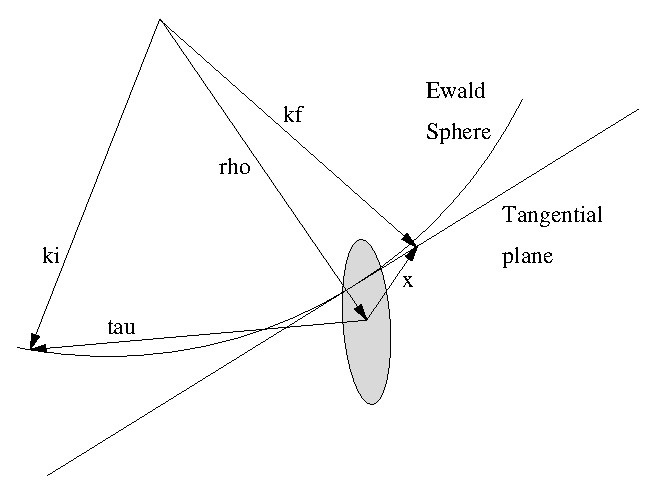
\includegraphics[width=0.7\textwidth]{figures/recip-detail}
  \end{center}
\caption{The scattering triangle in the single crystal.}
\label{fig:crystal-scattering-tri}
\end{figure}

The equation for the plane is
\begin{equation}
  \label{eq:crystal-tangent-plane}
    \boldsymbol{P}(\boldsymbol{t}) = \boldsymbol{o} + B \boldsymbol{t}, \qquad
    \boldsymbol{t} \in \mathbb{R}^2
\end{equation}
Here $B = (\boldsymbol{b}_1, \boldsymbol{b}_2)$ is a $3\times 2$ matrix
with the two generators for the plane $\boldsymbol{b}_1$ and
$\boldsymbol{b}_2$. These are (arbitrary) unit vectors in the plane,
being perpendicular to
each other and to the plane normal $\boldsymbol{n} =
\boldsymbol{\rho}/\rho$.

Each $\boldsymbol{t}$ defines a potential final wave vector
$\boldsymbol{k}_\textrm{f}(\boldsymbol{t}) = \boldsymbol{k}_\textrm{i} +
\boldsymbol{P}(\boldsymbol{t})$. The value of the 3-dimensional Gaussian
for this $\boldsymbol{k}_\textrm{f}$ is
\begin{equation}
  \label{eq:crystal-gauss-t-1}
  G(\boldsymbol{x}(\boldsymbol{t})) =
  \frac{1}{(\sqrt{2\pi})^3}\frac{1}{\sigma_1\sigma_2\sigma_3}
  e^{-\boldsymbol{x}(\boldsymbol{t})^\textrm{T} D \boldsymbol{x}(\boldsymbol{t})}
\end{equation}
where $\boldsymbol{x}(\boldsymbol{t}) = \boldsymbol{\tau} -
(\boldsymbol{k}_\textrm{i} - \boldsymbol{k}_\textrm{f}(\boldsymbol{t}))$ is
given in local coordinates for $\boldsymbol{\tau}$. It can be shown that
equation~(\ref{eq:crystal-gauss-t-1}) can be re-written as
\begin{equation}
  \label{eq:crystal-gauss-2}
  G(\boldsymbol{x}(\boldsymbol{t})) =
  \frac{1}{(\sqrt{2\pi})^3}\frac{1}{\sigma_1\sigma_2\sigma_3} e^{-\alpha}
  e^{-(\boldsymbol{t}-\boldsymbol{t}_0)^\textrm{T} M
    (\boldsymbol{t}-\boldsymbol{t}_0)}
\end{equation}
where $M = B^\textrm{T} D B$ is a $2 \times 2$ symmetric and positive
definite matrix, $\boldsymbol{t}_0 = -M^{-1}B^\textrm{T} D \boldsymbol{o}$
is a 2-vector, and $\alpha = -\boldsymbol{t}_0^\textrm{T} M
\boldsymbol{t}_0 + \boldsymbol{o}^\textrm{T} D \boldsymbol{o}$ is a real
number.  Note that this is a two-dimensional Gaussian (not necessarily
normalized) in $\boldsymbol{t}$ with center $\boldsymbol{t}_0$ and axis
defined by $M$.

To choose $\boldsymbol{k}_\textrm{f}$ we sample $\boldsymbol{t}$ from the
2-dimensional Gaussian distribution~(\ref{eq:crystal-gauss-2}). To do
this, we first construct the Cholesky decomposition of the matrix
$(\frac{1}{2}M^{-1})$. This gives a $2\times 2$ matrix $L$ such that $L
L^\textrm{T} = \frac{1}{2}M^{-1}$ and is possible since $M$ is symmetric
and positive definite. It is given by
$$
  L = \left(
  \begin{array}[c]{cc}
    \sqrt{\nu_{11}} & 0 \\
    \frac{\nu_{12}}{\sqrt{\nu_{11}}} & \sqrt{\nu_{22} - \frac{\nu_{12}^2}{\nu_{11}}}
  \end{array}\right)
\qquad\hbox{where }
  \frac{1}{2}M^{-1} = \left(
  \begin{array}[c]{cc}
    \nu_{11} & \nu_{12} \\
    \nu_{12} & \nu_{22}
  \end{array}\right)
$$
Now let $\boldsymbol{g} = (g_1, g_2)$ be two random numbers drawn form a
Gaussian distribution with mean 0 and standard deviation 1, and let
$\boldsymbol{t} = L\boldsymbol{g} + \boldsymbol{t}_0$. The probability
of a particular $\boldsymbol{t}$ is then
\begin{eqnarray}
  P(\boldsymbol{t})d\boldsymbol{t}
    &=& \frac{1}{2\pi}
      e^{-\frac{1}{2}\boldsymbol{g}^\textrm{T}\boldsymbol{g}} d\boldsymbol{g} \\
    &=& \frac{1}{2\pi}\frac{1}{\det L}
      e^{-\frac{1}{2}(L^{-1}(\boldsymbol{t}-\boldsymbol{t}_0))^\textrm{T}
          (L^{-1}(\boldsymbol{t}-\boldsymbol{t}_0))} d\boldsymbol{t} \\
    &=& \frac{1}{2\pi}\frac{1}{\det L}
      e^{-(\boldsymbol{t}-\boldsymbol{t}_0)^\textrm{T}
          M(\boldsymbol{t}-\boldsymbol{t}_0)} d\boldsymbol{t}
  \label{eq:crystal-gauss-prob-1}
\end{eqnarray}
where we used that
$\boldsymbol{g}=L^{-1}(\boldsymbol{t}-\boldsymbol{t}_0)$ so that
$d\boldsymbol{g} = \frac{1}{\det L}d\boldsymbol{t}$. This is just the
normalized form of~(\ref{eq:crystal-gauss-2}). Finally we set
$\boldsymbol{k}'_\textrm{f} = \boldsymbol{k}_\textrm{i} +
\boldsymbol{P}(\boldsymbol{t})$ and
$\boldsymbol{k}_\textrm{f} = (k_\textrm{i}/k'_f)\boldsymbol{k}'_\textrm{f}$ to
normalize the length of $\boldsymbol{k}_\textrm{f}$ to correct for the
(small) error introduced by approximating the Ewald sphere with a plane.

\subsection{Computing the total coherent cross-section}

To determine the total coherent scattering cross-section, the differential
cross-section must be integrated over the Ewald sphere:
$$
\sigma_\textrm{coh} = \int_\textrm{Ewald}
\left(\frac{d\sigma}{d\Omega}\right)_\textrm{coh.el.} d\Omega
$$
For small mosaic we may approximate the sphere with the tangential
plane, and we thus get from~(\ref{eq:crystal-cross-section})
and~(\ref{eq:crystal-gauss-2}):
\begin{eqnarray}
  \label{eq:crystal-coh-cs}
  \sigma_{\textrm{coh},\boldsymbol{\tau}} &=& \int N\frac{(2\pi)^3}{V_0}
        G(\boldsymbol{\tau} - \boldsymbol{\kappa})
         |F_{\boldsymbol{\tau}}|^2 d\Omega \\
  &=& \frac{1}{\boldsymbol{k}_i^2} N\frac{(2\pi)^3}{V_0}
         \frac{1}{(\sqrt{2\pi})^3}\frac{e^{-\alpha}}{\sigma_1\sigma_2\sigma_3}
         |F_{\boldsymbol{\tau}}|^2
         \int e^{-(\boldsymbol{t}-\boldsymbol{t}_0)^\textrm{T} M
         (\boldsymbol{t}-\boldsymbol{t}_0)}
         d\boldsymbol{t} \\
  &=& \det(L) \frac{1}{\boldsymbol{k}_i^2} N\frac{(2\pi)^{3/2}}{V_0}
         \frac{e^{-\alpha}}{\sigma_1\sigma_2\sigma_3}
         |F_{\boldsymbol{\tau}}|^2
         \int e^{-\frac{1}{2}\boldsymbol{g}^\textrm{T}\boldsymbol{g}}
         d\boldsymbol{g} \\
  &=& 2\pi\det(L) \frac{1}{\boldsymbol{k}_i^2} N\frac{(2\pi)^{3/2}}{V_0}
         \frac{e^{-\alpha}}{\sigma_1\sigma_2\sigma_3}
         |F_{\boldsymbol{\tau}}|^2 \\
  &=& \frac{\det(L)}{\boldsymbol{k}_i^2} N\frac{(2\pi)^{5/2}}{V_0}
         \frac{e^{-\alpha}}{\sigma_1\sigma_2\sigma_3}
         |F_{\boldsymbol{\tau}}|^2 \\
  \sigma_\textrm{coh} &=& \sum_{\boldsymbol{\tau}} \sigma_{\textrm{coh},\boldsymbol{\tau}}
\end{eqnarray}
As before, we let $\boldsymbol{g} = L^{-1}(\boldsymbol{t} -
\boldsymbol{t}_0)$ so that $d\boldsymbol{t} = \det(L) d\boldsymbol{g}$.

\paragraph{Neutron weight factor adjustment}

We now calculate the correct neutron weight adjustment for the Monte
Carlo choices made. In three cases is a Monte Carlo choice made with a
probability different from the probability of the corresponding physical
event: When deciding whether to transmit the neutron or not, when
simulating absorption, and when selecting the reciprocal lattice vector
$\boldsymbol{\tau}$ to scatter from.

If the user has choosen a fixed transmission probability $f(\textrm{
  transmit}) = p_\textrm{transmit}$, the neutron weight must be adjusted by
$$ \pi(\textrm{transmit}) = \frac{P(\textrm{transmit})}{f(\textrm{transmit})}
$$
where $P(\textrm{transmit}) = \exp(-\frac{\sigma_\textrm{tot}}{V_0}\ell)$ is
the physical transmission probability. Likewise, for non-transmission
the adjustment is
$$ \pi(\textrm{no~transmission}) = \frac{1-P(\textrm{transmit})}{1-f(\textrm{transmit})}.
$$

Absorption is never explicitly simulated, so the Monte Carlo probability
of coherent or incoherent scattering is
$f(\textrm{coh})+f(\textrm{inc}) = 1$.
The physical probability of coherent or incoherent scattering is
$$ P(\textrm{coh})+P(\textrm{inc}) = \frac{\sigma_\textrm{coh} + \sigma_\textrm{
    inc}}{\sigma_\textrm{tot}}, $$
so again a weight adjustment $\pi(\textrm{coh}|\textrm{inc}) = \Pi(\textrm{
    coh}|\textrm{inc})/f(\textrm{coh}|\textrm{inc})$ is needed.

When choosing the reciprocal lattice vector $\boldsymbol{\tau}$ to
scatter from, the relative probability for $\boldsymbol{\tau}$ is
$r_{\boldsymbol{\tau}} = \sigma_{\textrm{
    coh},\boldsymbol{\tau}}/|F_{\boldsymbol{\tau}}|^2$. This is done to
get better statistics for weak reflections. The Monte Carlo probability
for the reciprocal lattice vector $\boldsymbol{\tau}$ is thus
$$ f(\boldsymbol{\tau}) =
\frac{r_{\boldsymbol{\tau}}}{\sum_{\boldsymbol{\tau}} r_{\boldsymbol{\tau}}}
$$
whereas the physical probability is $P(\boldsymbol{\tau}) = \sigma_{\textrm{
    coh},\boldsymbol{\tau}}/\sigma_\textrm{coh}$. A weight adjustment is
thus needed of
$$
\pi(\boldsymbol{\tau}) =
 \frac{P(\boldsymbol{\tau})}{f(\boldsymbol{\tau})} =
 \frac{\sigma_{\textrm{coh},\boldsymbol{\tau}}
  \sum_{\boldsymbol{\tau}} r_{\boldsymbol{\tau}}}
 {\sigma_\textrm{coh} \; r_{\boldsymbol{\tau}}}.$$

In most cases, however, only one reflection is possible, whence $\pi=1$.

\subsection{Implementation details}
\label{s:Single_crystal_implement}

The equations describing \textbf{Single\_crystal} are quite
complex, and consequently the code is fairly sizeable. Most of it is
just the expansion of the vector and matrix equations in individual
coordinates, and should thus be straightforward to follow.

The implementation pre-computes a lot of the necessary values in the
\texttt{INITIALIZE} section. It is thus actually very efficient despite
the complexity. If the list of reciprocal lattice points is big,
however, the search through the list will be slow. The precomputed data
is stored in the structures \texttt{hkl\_info} and in an array of
\texttt{hkl\_data} structures (one for each reciprocal lattice point in
the list). In addition, for every neutron event an array of
\texttt{tau\_data} is computed with one element for each reciprocal
lattice point close to the Ewald sphere. Except for the search for
possible $\boldsymbol{\tau}$ vectors, all computations are done in local
coordinates using the matrix $U$ to do the necessary transformations.

The list of reciprocal lattice points is specified in an ASCII data
file. Each line contains seven numbers, separated by white space. The
first three numbers are the $(h,k,l)$ indices of the reciprocal lattice
point, and the last number is the value of the structure factor
$|F_{\boldsymbol{\tau}}|^2$, in barns. The middle three numbers are not
used and may be omitted; they are nevertheless recommended since this makes
the file format compatible with the output from the Crystallographica
program~\cite{crystallographica}.
Any line beginning with any character of \verb+#;/%+ is considered to be a
comment, and lines which can not be read as vectors/matrices are ignored.

The column signification may also explicitely be set in the data file header using any of the lines:
\begin{lstlisting}
  #column_h <index of the Bragg Qh column>
  #column_k <index of the Bragg Qk column>
  #column_l <index of the Bragg Ql column>
  #column_F2 <index of the squared str. factor '|F|^2' column [b]>
  #column_F  <index of the structure factor norm '|F|' column>
\end{lstlisting}

Other component parameters may as well be specified in the data file
header with lines e.g.:
\begin{lstlisting}
  #sigma_abs <value of Absorption cross section [barns]>
  #sigma_inc <value of Incoherent cross section [barns]>
  #Delta_d/d <value of Delta_d/d width for all lines>
  #lattice_a <value of the a lattice parameter [Angs]>
  #lattice_a <value of the b lattice parameter [Angs]>
  #lattice_a <value of the c lattice parameter [Angs]>
  #lattice_aa <value of the alpha lattice angle [deg]>
  #lattice_bb <value of the beta  lattice angle [deg]>
  #lattice_cc <value of the gamma lattice angle [deg]>
\end{lstlisting}

Example data \verb+*.lau+ files are given in directory \verb+MCSTAS/data+.

These files contain an extensive self-documented header defining most the sample parameters, so that only the file name and mosaicity should be given to the component:
\begin{lstlisting}
  Single_crystal(xwidth=0.01, yheight=0.01, zdepth=0.01,
    mosaic = 5, reflections="YBaCuO.lau")
\end{lstlisting}

Powder files from ICSD/LAZY \cite{icsd_ill} and Fullprof \cite{Fullprof}
may also be used (see Table \ref{t:powders-data}, page \pageref{t:powders-data}).
We do not recommend to use these as the equivalent $\vec q$ vectors are superposed, not
all Bragg spots will be simulated, and the intensity will not be scaled by the
multiplicity for each spot.

   \newpage
\section{Molecule\_2state: Excitable time-dependent sample model}
\index{Samples!liquid, diffraction}
\index{DFT}
\index{time resolved}
\label{molecule_2state}

\mcdoccomp{samples/Molecule_2state.parms}

Further Documentaion pending
 \newpage
%\input{samples/saxs.tex}             \newpage
%\input{samples/absorption_phantom.tex} \newpage
%\input{phonon.tex}           \newpage
%\input{LSCO.tex}            \newpage
%\input{isotropic_sqw.tex}
